\documentclass[main.tex]{subfiles}

\begin{document}

\subsection{Terzo esercizio}

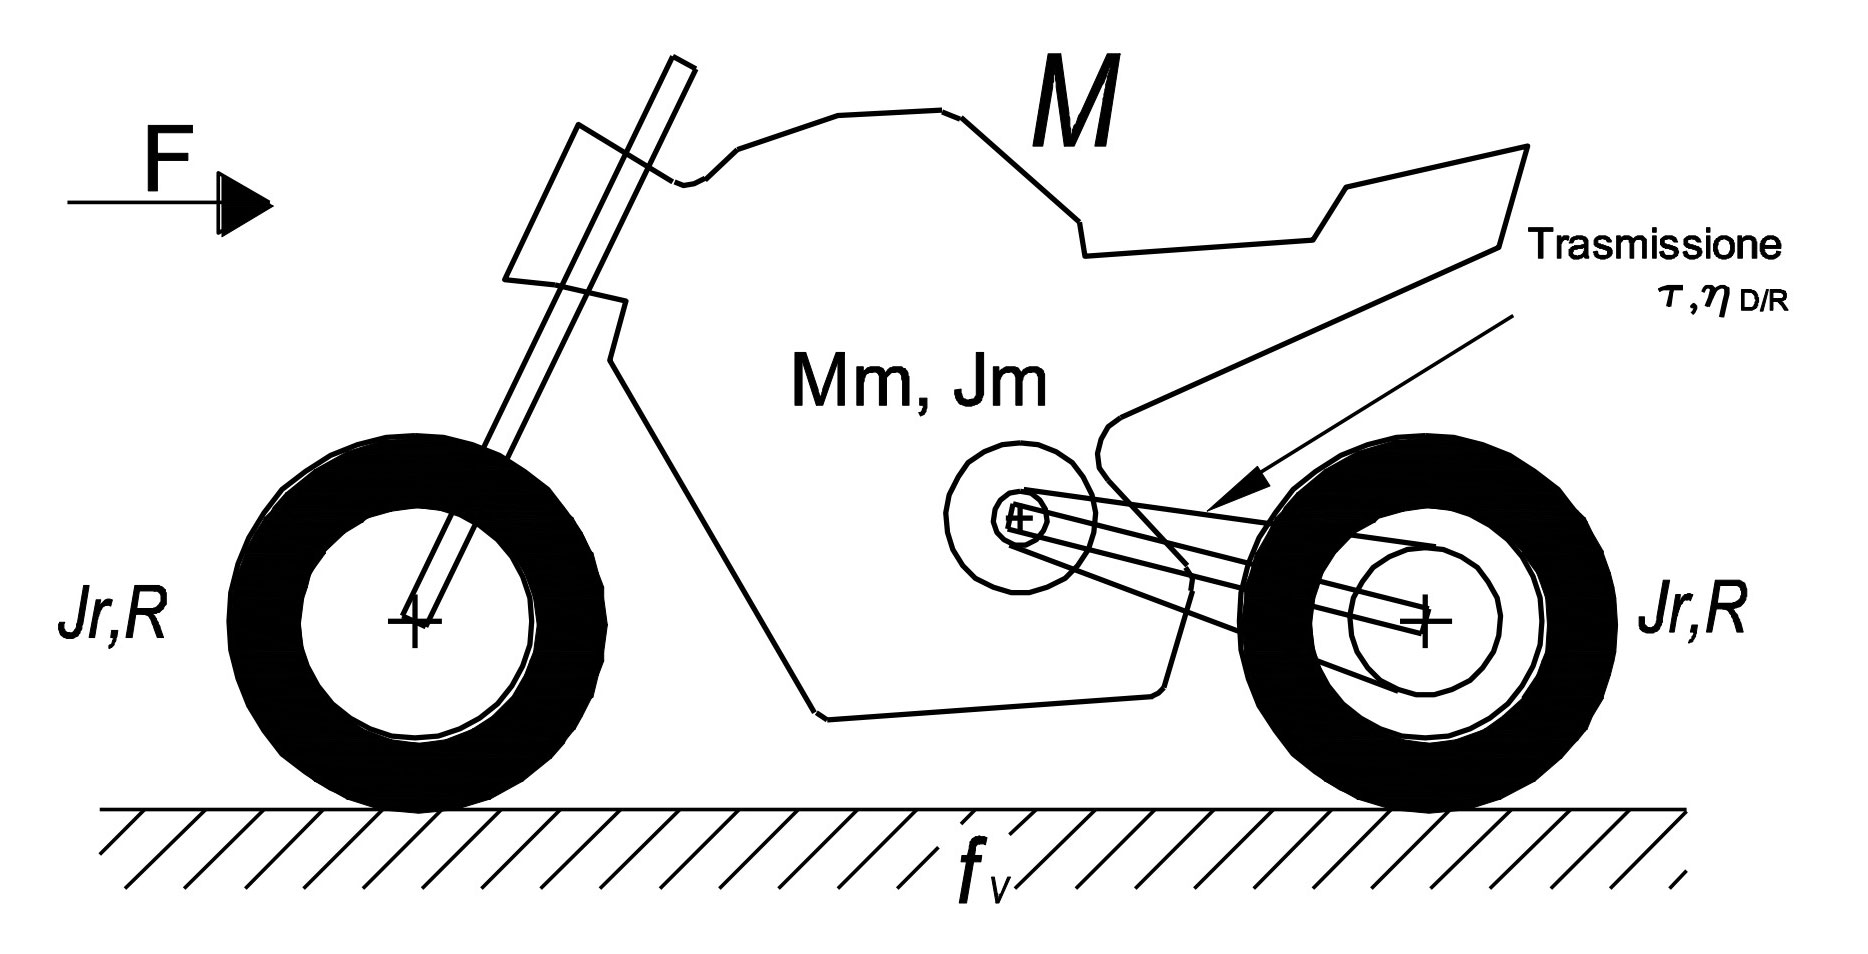
\includegraphics[width=\textwidth]{2014-2409-3.jpg}

\[
  M = 250\,kg\quad
  J_r = 0.6\,kgm^2\quad
  R = 0.25\,m\quad
  J_m = 0.1\,kgm^2\quad
  f_v = 0.03
\]

\[
  k = 0.3\,kg/m\quad
  \tau = \dfrac{1}{6}\quad
  \mu_D = 0.9 \quad
  \mu_R = 0.8
\]

Il veicolo rappresentato in figura, posto nel piano verticale, procede su strada piana. Il motore, avente momento d'inerzia $J_m$ e coppia motrice $M_m$, è collegato alla ruota posteriore mediante una trasmissione a catena di caratteristiche note (rapporto di trasmissione $\tau$, rendimento in moto diretto $\mu_D$, rendimento in moto retrogrado $\mu_R$). Al veicolo è applicata una forza aerodinamica resistente $F = kv^2$. Si consideri la resistenza al rotolamento nel contatto tra ruote e asfalto (coefficiente $f_V$). Si trascurino le masse non esplicitamente indicate nel disegno.
Si chiede di:

\begin{enumerate}
\item Calcolare la velocità del veicolo a regime, nota la coppia motrice $M_m$ pari a 15 Nm.
\item Partendo dalla situazione del punto 1, calcolare l’accelerazione del veicolo a fronte di una coppia motrice $M_m$ erogata dal motore pari a 30 Nm.
\end{enumerate}

\clearpage

\subsection{Soluzione terzo esercizio}

\subsubsection{Primo punto}

\paragraph{Legami cinematici} Data una velocità angolare motrice $\omega_m$, posso andare a definire la velocità con cui il veicolo si muove come:

\[
  v = R\omega_r = R\tau\omega_m
\]

\paragraph{Potenza motrice}

\[
  W_m = M_m\omega_m
\]

\paragraph{Potenza resistente} La potenza resistente è composta da tutte le forze ed attriti agenti sul sistema. In questo caso esse sono:

\begin{enumerate}
\item Forza peso $F_g$ della massa M è contro bilanciata da una forza normale uguale ed opposta.
\item Forza areodinamica resistente $F_{aria}$, che forma un angolo di $\pi$ con la velocità.
\item Forza di attrito volvente $F_v$, che forma un angolo di $\pi$ con la velocità.
\end{enumerate}



Risolvo il \textit{prodotto scalare} tramite la formula $|a||b|\cos\theta$ con $\theta$ definito come l'angolo tra i due vettori, ed ottengo:

\begin{align*}
  W_r &= \vec{F}_{aria}\bullet\vec{v} + \vec{F}_v\bullet\vec{v}\\
    &= F_{aria}v\cos\pi + F_vv\cos\pi\\
    &= - F_{aria}v  - F_vv\\
\end{align*}

\subparagraph{Forza d'attrito volvente} La forza d'attrito volvente è definita come la reazione normale del piano $\vec{N}$ moltiplicata per il coefficiente d'attrito $f_v$. In questo caso, la reazione normale risulta uguale, in modulo, alla forza peso.

\[
  F_v = F_gf_v = Mgf_v
\]

\subparagraph{Forza areodinamica resistente} Viene definita tramite la formula fornita dal testo:

\[
  F_{aria} = kv^2
\]

Sostituisco i termini nell'espressione della potenza resistente ed ottengo:

\[
  W_r = -kv^3 - Mgf_vv
\]

\paragraph{Identificazione del tipo di moto}
Siamo in condizione di regime, per cui la variazione di energia cinetica è nulla. Per identificare il tipo di moto uso la seguente disequazione:

\[
  W_r > 0
\]

Se essa risulta vera, il moto è \textbf{retrogrado}, altrimenti diretto:

\[
  -kv^3 - Mgf_vv > 0
\]

Siccome tutti i coefficienti dell'equazione hanno segno negativo, l'equazione è falsa. Il moto è quindi \textbf{diretto}.

\paragraph{Potenze perduta}
Vista la condizione di regime e di moto diretto, uso la formula corrispondente per calcolare la potenza perduta:

\[
  W_p = -(1-\mu_D)W_m
\]

\paragraph{Bilancio di potenze}
Utilizzo il bilancio delle potenze e risolvo in funzione della velocità:

\begin{equation}
  W_m + W_r + W_p = 0
\end{equation}

\begin{equation}
  W_m + W_r - (1-\mu_D)W_m = 0
\end{equation}

Semplifico la potenza motrice:

\begin{equation}
  W_r +\mu_DW_m = 0
\end{equation}

Sostituisco le espressioni:

\begin{equation}
  M_m\omega_m\mu_D -kv^3 - Mgf_vv = 0
\end{equation}

Sostituisco il legame cinematico tra velocità e velocità angolare $v = R\tau\omega_m$:

\begin{equation}
  \dfrac{M_m\mu_Dv}{R\tau} -kv^3 - Mgf_vv = 0
\end{equation}

Semplifico la velocità:

\begin{equation}
  \dfrac{M_m\mu_D}{R\tau} -kv^2 - Mgf_v = 0
\end{equation}

Risolvo in funzione di $v$:

\begin{equation}
   v  = \sqrt{\dfrac{\dfrac{M_m\mu_D}{R\tau} - Mgf_v}{k}}
\end{equation}

Per le condizioni di moto, la velocità deve essere positiva, per cui solo la risposta positiva può essere accettata.

\begin{equation}
  v = 28.9\,m/s
\end{equation}

\subsubsection{Secondo punto}
Non siamo più in condizioni di regime, ma di transitorio. È dunque necessario calcolare la variazione di energia cinetica del sistema.

\[
  E_c = \dfrac{1}{2}Mv^2 + \dfrac{1}{2}J_r(\tau\omega_m)^2 + \dfrac{1}{2}J_r(\tau\omega_m)^2 + \dfrac{1}{2}J_m\omega_m^2
\]

\[
  E_c = \dfrac{1}{2}M(\tau R\omega_m)^2 + 2\dfrac{1}{2}J_r(\tau\omega_m)^2 + \dfrac{1}{2}J_m\omega_m^2
\]

\[
  E_c = \omega_m^2(\dfrac{1}{2}M\tau^2R^2 + J_r\tau^2 + \dfrac{1}{2}J_m)
\]

Derivo l'espressione ed ottengo:

\[
  \dfrac{dE_c}{dt} = \omega_m\dot{\omega}_m(M\tau^2R^2 + 2J_r\tau^2 + J_m)
\]

\paragraph{Verifico il tipo di moto}
Verrebbe istintivo dire che siamo sempre in condizioni di moto diretto, ma verifico comunque il tipo di moto:

\[
  W_r - \dfrac{dE_{c_r}}{dt} > 0
\]

\[
  -kv^3 - Mgf_vv -\omega_m\dot{\omega}_m(M\tau^2R^2 + 2J_r\tau^2) > 0
\]

Nuovamente i coefficienti sono tutti negativi, e il moto non può che essere diretto.

\paragraph{Potenza perduta}
Siccome siamo in condizioni di transitorio, è necessarrio includere la variazione nel tempo dell'energia cinetica del motore \footnote{perché siamo in condizioni di moto \textit{diretto}, in condizioni di moto \textit{retrogrado} si include la variazione di energia cinetica resistente.} nella formula della potenza perduta:

\[
  W_p = -(1-\mu_D)(W_m - \dfrac{dE_{c_m}}{dt})
\]

\paragraph{Bilancio di potenze}
\setcounter{equation}{0}
\begin{equation}
  W_m + W_r + W_p = \dfrac{dE_c}{dt}
\end{equation}

\begin{equation}
  W_m + W_r - (1-\mu_D)(W_m - \dfrac{dE_{c_m}}{dt}) = \dfrac{dE_c}{dt}
\end{equation}

Semplifico l'espressione:

\begin{equation}
  W_m + W_r - (1-\mu_D)(W_m - \dfrac{dE_{c_m}}{dt}) = \dfrac{dE_{c_m}}{dt}  + \dfrac{dE_{c_r}}{dt}
\end{equation}

\begin{equation}
  W_m + W_r - W_m + \dfrac{dE_{c_m}}{dt} + \mu_D(W_m - \dfrac{dE_{c_m}}{dt}) = \dfrac{dE_{c_m}}{dt}  + \dfrac{dE_{c_r}}{dt}
\end{equation}

\begin{equation}
  W_r + \mu_D(W_m - \dfrac{dE_{c_m}}{dt}) = \dfrac{dE_{M_r}}{dt}
\end{equation}

\begin{equation}
  W_r + \mu_DW_m  = \dfrac{dE_{M_r}}{dt} + \mu_D\dfrac{dE_{c_m}}{dt}
\end{equation}

\begin{equation}
  -kv^3 - Mgf_vv + \mu_DM_m\omega_m  = \omega_m\dot{\omega}_m(M\tau^2R^2 + 2J_r\tau^2 + \mu_DJ_m)
\end{equation}

Sostituisco col legame cinematico $v = R\tau\omega_m$:

\begin{equation}
  -kv^2R\tau\omega_m - Mgf_vR\tau\omega_m + \mu_DM_m\omega_m  = \omega_m\dot{\omega}_m(M\tau^2R^2 + 2J_r\tau^2 + \mu_DJ_m)
\end{equation}

Semplifico $\omega_m$:

\begin{equation}
  -kv^2R\tau - Mgf_vR\tau + \mu_DM_m  = \dot{\omega}_m(M\tau^2R^2 + 2J_r\tau^2 + \mu_DJ_m)
\end{equation}

\begin{equation}
  -kv^2R\tau - Mgf_vR\tau + \mu_DM_m  = \dot{\omega}_m(\tau^2(MR^2 + 2J_r) + \mu_DJ_m)
\end{equation}

\begin{equation}
 \dot{\omega}_m =   \dfrac{\mu_DM_m  -kv^2R\tau - Mgf_vR\tau}{\tau^2(MR^2 + 2J_r) + \mu_DJ_m}
\end{equation}

\begin{equation}
   \dot{\omega}_m = 24.2\,rad/s^2
\end{equation}

\begin{equation}
   a = R\tau\dot{\omega} = 1.01\,m/s^2
\end{equation}

\end{document}
